\section{Applikation}                                   
I følgende afsnit gøres der rede for beslutningerne i forhold til udvikling af applikationen.

\subsection{Styresystem}
Der findes forskellige styresystemer til mobiltelefoner i dag. De to mest brugte er dog iOS \cite{iOS} og Android. \cite{Android} \\
IOS er Apples eget styresystem som er udviklet i forhold til deres mobile og tablet devices. \\
Android er et stort open source project som bliver brugt på ca. 80\% af alle mobile og tablet devices i dag. Der findes forskellige versioner af Android styresystemet alt efter hvilken producent der har leveret devices. \\
Nogle af de kendte Android device leverendører er firmaer som Samsung, Huawei og HTC. De har alle en Android Core i deres styresystemer, men har alle også videre udviklet styresystemet, så det passer specifikt til deres devices.

Rambøll ønskede en applikation udviklet til iOS. Til en workshop med Rambøll, fandt vi ud af at der også var ansatte som bruger Android. Derfor blev der aftalt at udvikle cross-platform.

\subsection{Cross-platform udviklingsværktøjer}
I denne sektion vil der være en kort beskrivelse af nogle cross-platform udviklingsværktøjer.

\subsubsection{Xarmarin}
Xarmarin tilbyder en cross-platform, hvor der udviklet i C\#\cite{CSharp} og XAML\cite{XAML}.
Features Xarmarin tilbyder:
\begin{itemize}[-]
	\item Integreret i Visual Studio
	\item Fuld API Access til både iOS og Android
	\item Deling af kode
\end{itemize}

\subsubsection{PhoneGap}
PhoneGap er en platform udviklet af Adobe\cite{Adobe}. Her bruges teknologier som HTML5\cite{HTML5}, JavaScripts\cite{JavaScript} og CSS\cite{CSS}. \\
Deres platform tilbyder nogle bonus features som:
\begin{itemize}[-]
	\item Build server
	\item Easy share af applikationen 
	\item Mulitple plug-ins !!! Plug in i ordforklaringen
\end{itemize}

\clearpage

\subsubsection{Corona}
Corona tilbyder en cross-platform, hvor der udviklet i Lua scripting \cite{Lua}.
\begin{itemize}[-]
	\item Real time simulering
	\item Live testing
	\item Mange plug-in muligheder
\end{itemize}

\subsection{Valg af cross-platform udviklingsværktøj}
I følgende afsnit redegøres for de beslutninger der tages angående valg af Firebase. \\

Der var et lille kendskab til Xarmarin fra et tidligere projekt lavet på Ingeniør Højskolen. \\
Xarmarin giver mulighed for at skrive i C\# som er et sprog der er blevet undervist i på skolen og er et højniveau sprog. \\
Xarmarin blev i februar 2016 opkøbt af Microsoft, hvilket betyder at det siden da har været en integreret del af Microsoft Visual Studio, som er det fortrukne udviklingsværktøj.\\
Developer dokumentationen for Xarmarin er også et plus. Hvis man sidder med et problem, har Xarmarin lavet en meget grundig dokumentation, hvor man kan finde eksempler og guides til hvordan forskellige dele i en applikaiton skal programmeres.

\subsection{Xarmarin}
I denne sektion vil der komme en mere dybdegående beskrivelse af hvordan Xarmarin platformen er bygget op.

En af fordelene ved at skrive i Xarmarin, er at man kan dele C\# kode for de forskellige applikationer.
På billedet herunder kan man se hvordan at User Iterface koden og App Logic koden, er delt på tværs af alle tre enheder. Man skal altså kun skrive sin App Logic og User Interface én gang og virke på både iOS, Android og Windows.
\begin{figure}[H]
	\centering
	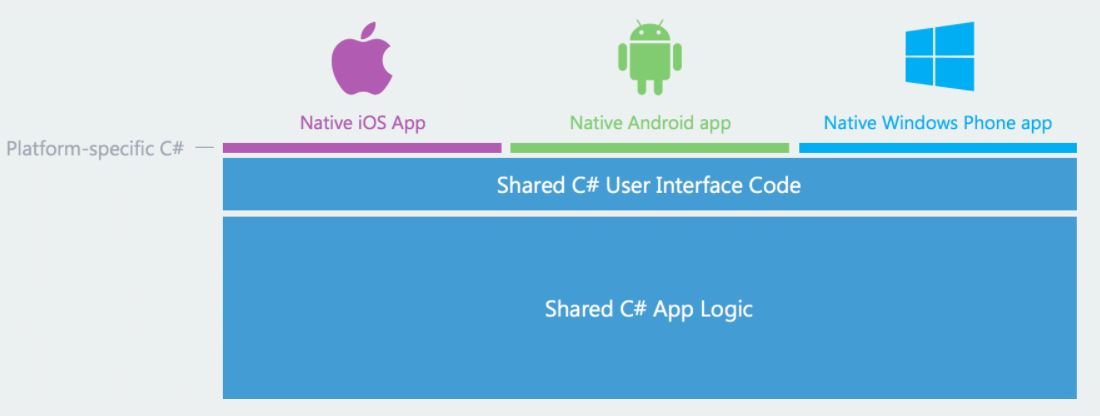
\includegraphics[width=1\linewidth]{Applikation/XarmarinShare.JPG}
	\caption{Kode deling i Xarmarin}
	\label{fig:CodeShare}
\end{figure}

\clearpage

Xarmarin kommer både med Xarmarin.iOS og Xarmarin.Android. Hvad dette gør er at når du kompiler koden, komplier den ned til native kode. IOS delen vil blive kompileret til ARM assembly, så ens app er native binære platform. Android kompileres så den kører native Android APK. Så man vil får kompileret koden så den passer til den specifike enhed, man vil bruge. \\
Xarmarin er baseret på C\# og ved hjælp af Xarmarin.iOS og Xarmarin.Android er det muligt at kalde binde det sammen med den eksisterende kode i både iOS og Android, gennem Xarmarins automatiske binding generator. \\
Der bliver i både Xarmarin.iOS og Xarmarin.Android givet muligheder for at forbinde til alle API'er der er nødvendige. \\

\begin{figure}[H]
	\centering
	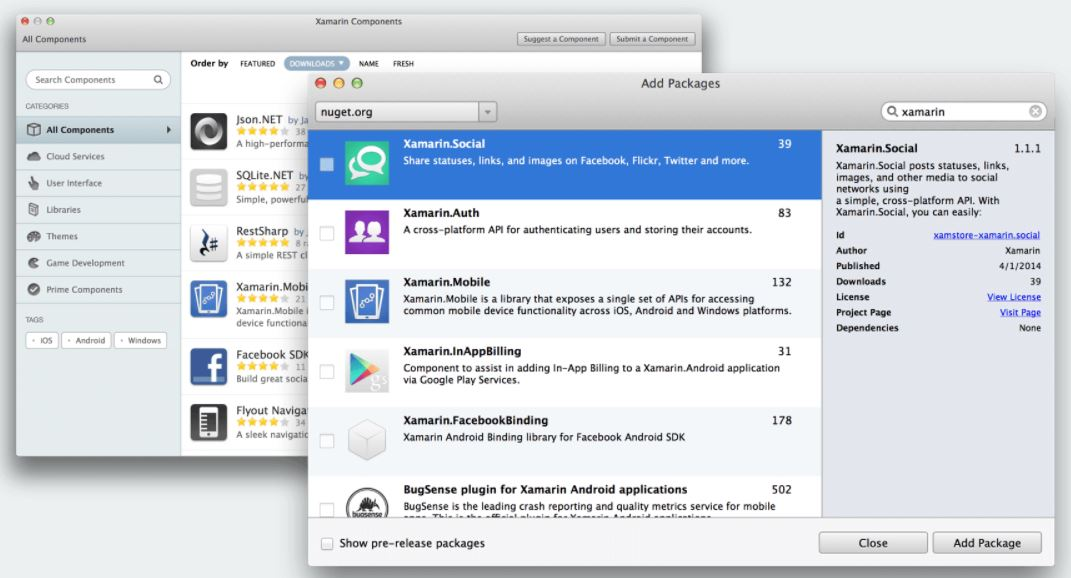
\includegraphics[width=0.7\linewidth]{Applikation/NuGet.JPG}
	\caption{NuGet og Xarmarin Componet Store}
	\label{fig:NuGet}
\end{figure}
Xarmarin tilbyder også en masse ekstra komponenter som kan integreres i ens applikation. Det kan være alt fra web api'er til sikkerheds features.

\clearpage